We conduct experiments to illustrate the properties of the OFDM system. The experiment setup is as follows.
\begin{itemize}
    \item The experiment is done in MATLAB.
    \item The modulation scheme is 16-QAM.
    \item The OFDM system has 64 subcarriers.
    \item There are $10^5$ iterations. Each iteration has 3 OFDM symbols.
    \item The cyclic prefix is added in between OFDM symbols and its length is either 3 or 16.
    \item The Channel condition is either AWGN or Rayleigh fading. For the Rayleigh fading channel, the channel is set to have 5 taps with the delay spread being $[0, 3, 5, 6, 8]$ and the channel power being $[0, -8, -17, -21, -25]$.
    \item We evaluate the average Bit Error Rate (BER) vs.\. the EbN0 (dB) over iteration with EbN0 being $[0:5:30]$.
    \item The simulation result is shown in~\cref{fig:BER}.
\end{itemize}

\begin{figure}[!htbp]
    \centering
    \begin{subfigure}[t]{0.5\linewidth}
        \centering
        \caption{AWGN Channel with 3-tap CP}
        \includegraphics[width=\linewidth]{AWGN_3.eps}
        \label{fig:AWGN_3}
    \end{subfigure}%
    % ~
    \begin{subfigure}[t]{0.5\linewidth}
        \centering
        \caption{AWGN Channel with 16-tap CP}
        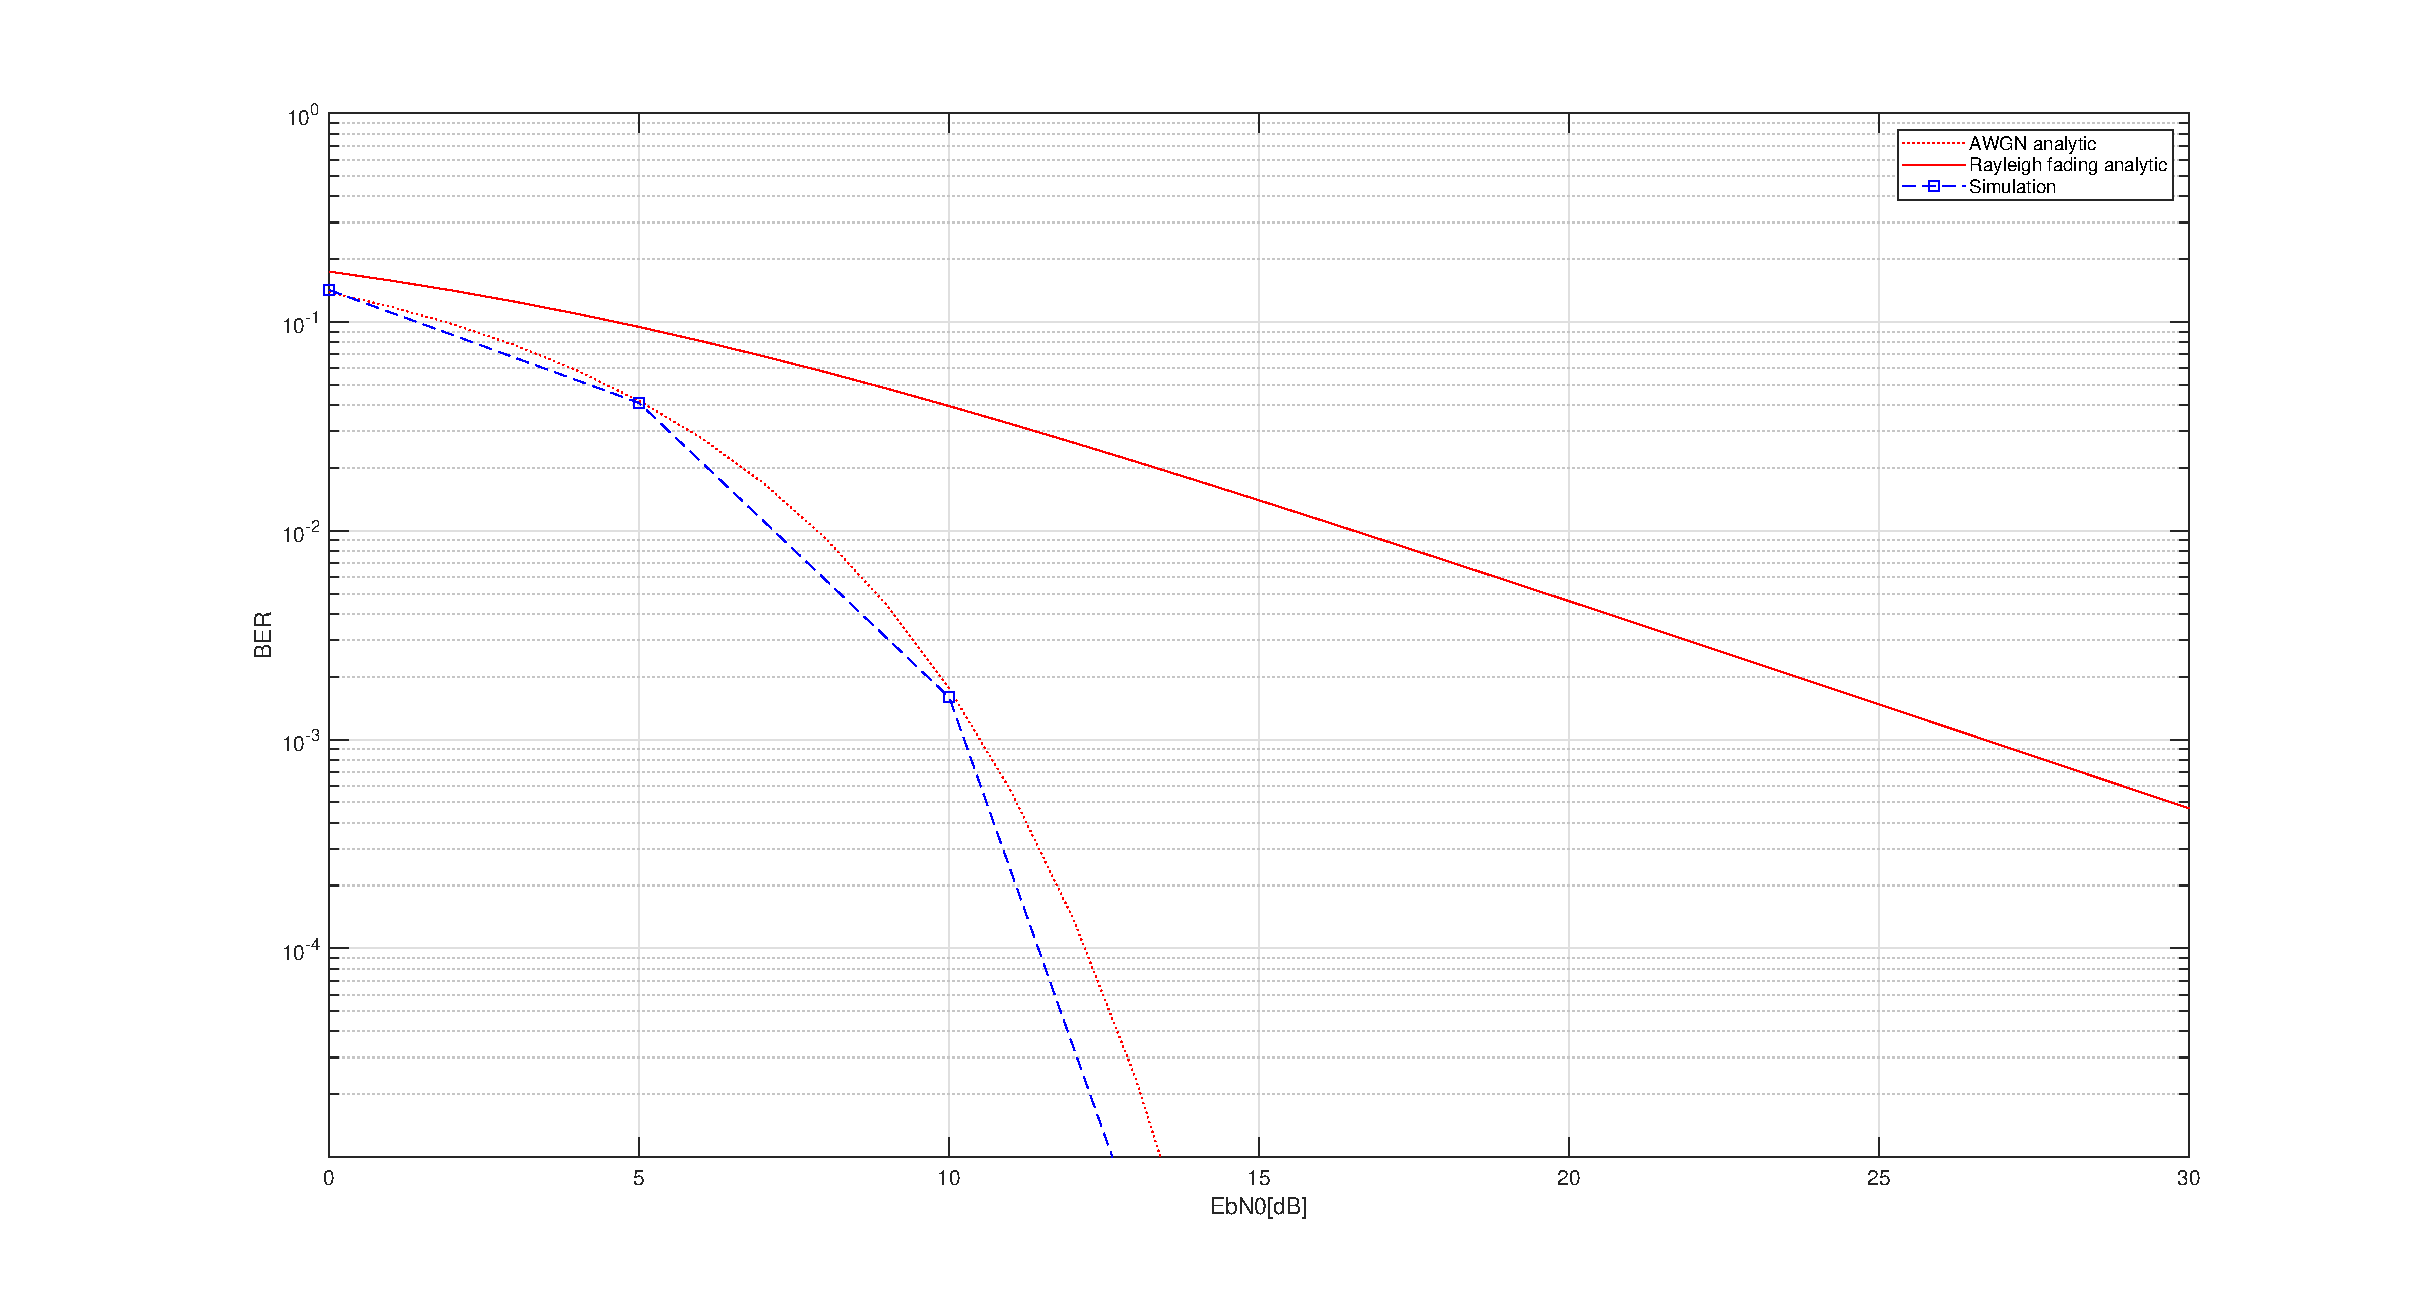
\includegraphics[width=\linewidth]{AWGN_16.eps}
        \label{fig:AWGN_16}
    \end{subfigure}%
    \\ %
    \begin{subfigure}[t]{0.5\linewidth}
        \centering
        \caption{Rayleigh Channel with 3-tap CP}
        \includegraphics[width=\linewidth]{Rayleigh_3.eps}
        \label{fig:Rayleigh_3}
    \end{subfigure}%
    % ~
    \begin{subfigure}[t]{0.5\linewidth}
        \centering
        \caption{Rayleigh Channel with 16-tap CP}
        \includegraphics[width=\linewidth]{Rayleigh_16.eps}
        \label{fig:Rayleigh_16}
    \end{subfigure}%
    \caption{BER performance for OFDM system with 16-QAM. The~\cref{fig:AWGN_3,fig:AWGN_16} are for AWGN channel. The different CP length does not affect the simulation results since the flat fading has constant complex gain on the transmitted signal. The~\cref{fig:Rayleigh_3,fig:Rayleigh_16} are for Rayleigh fading channel with 5 taps. The simulation results show that the BER exceeds the analytical result if the CP length is shorter than the delay taps, while the BER will be closed to the analytical result if the CP length is longer than the delay taps. The result implies that the OFDM system is only subject to flat fading as long as the CP length is longer than the channel delay spread.}
    \label{fig:BER}
\end{figure}